% GENERATED by build_chapters.py; edit docs/report/chapters, not this file

\chapter{Evaluation and Results}

\section{How to read this chapter}

The project ran nine studies, each on the Kaggle machine or against the live pipeline. This chapter gives them in the order they answer questions about the healer: first which model file to load, then how to make it fast, then what output format to ask for, then how often the fix is right, and last how the whole pipeline behaves live. Each section states the question, the method, the decision rule when the results document names one, the headline numbers and the conclusion.

Every number comes from a results document in \texttt{docs/\allowbreak{}results/\allowbreak{}} or \texttt{docs/\allowbreak{}old/\allowbreak{}}, with the file named after it in brackets. Where saved data exists under \texttt{eval/\allowbreak{}runs/\allowbreak{}}, we recomputed the headline numbers from it. A section says so when the data confirmed the document, and says so when it did not or when the data was not kept. Disagreements between documents are named where they occur and collected in the last table.

\section{The evaluation harness}

The \texttt{eval/\allowbreak{}} folder holds the test cases, the scorers, the scripts that build Kaggle kernels from them, and the saved results in \texttt{eval/\allowbreak{}runs/\allowbreak{}}.

\textbf{Cases.} There are 5 control cases (\texttt{eval/\allowbreak{}cases/\allowbreak{}eval\_\allowbreak{}cases.\allowbreak{}json}), 6 hard single-file cases (\texttt{eval/\allowbreak{}cases/\allowbreak{}hard\_\allowbreak{}cases.\allowbreak{}json}) and 6 multi-file cases (\texttt{eval/\allowbreak{}cases/\allowbreak{}multifile\_\allowbreak{}cases.\allowbreak{}json}). The control cases are the five breakages the live runner pushes to the demo repository: a missing \texttt{app} line, a misspelled method, a missing \texttt{require}, a missing closing brace and a wrong status check. The hard cases come from the same file, but the CI log no longer points at the bug. The multi-file cases use the demo app's \texttt{src/\allowbreak{}app.\allowbreak{}js}, \texttt{src/\allowbreak{}format.\allowbreak{}js} and \texttt{test/\allowbreak{}api.\allowbreak{}test.\allowbreak{}js} (source: \texttt{docs/\allowbreak{}results/\allowbreak{}SHIPPED\_\allowbreak{}QUALITY\_\allowbreak{}EVAL.\allowbreak{}md}, \texttt{docs/\allowbreak{}results/\allowbreak{}MULTIFILE\_\allowbreak{}EVAL.\allowbreak{}md}). We counted the cases in the three JSON files.

\textbf{Same code as production.} The later studies do not paraphrase the pipeline. They run the real node code from \texttt{tools/\allowbreak{}nodes/\allowbreak{}} (\texttt{build\_\allowbreak{}ai\_\allowbreak{}prompt.\allowbreak{}js}, \texttt{extract\_\allowbreak{}ai\_\allowbreak{}response.\allowbreak{}js}, and for multi-file cases \texttt{Pick Candidate Files}) under \texttt{node}, send the request body unchanged to the model, and apply the reply with the real extraction node, so its exactly-once and syntax gates count (source: \texttt{docs/\allowbreak{}results/\allowbreak{}SHIPPED\_\allowbreak{}QUALITY\_\allowbreak{}EVAL.\allowbreak{}md}, \texttt{docs/\allowbreak{}results/\allowbreak{}MODEL\_\allowbreak{}BAKEOFF.\allowbreak{}md}).

\textbf{What "healed" means.} Live, a case counts as healed when three things hold: the file on the pull request branch parses, it is byte-identical to the known-good file, and the real smoke test passes (source: \texttt{docs/\allowbreak{}results/\allowbreak{}GOLIVE\_\allowbreak{}RESULTS.\allowbreak{}md}). In the offline studies the test result comes first. The patched file is run as the real smoke test (\texttt{node test.\allowbreak{}js} with express), and exit code 0 means healed; for multi-file cases the full \texttt{npm test} must pass. Byte equality with the golden file is kept as a second, stricter column, and a \texttt{mustnot} pattern flags answers that cheat (source: \texttt{eval/\allowbreak{}shipped\_\allowbreak{}quality\_\allowbreak{}eval.\allowbreak{}py}, function \texttt{score}). Before any GPU time, a preflight proves that the golden file passes and that every broken file fails with exit code 1.

\textbf{Why test first, byte-exact second.} The alternative-quant study found a case, \texttt{route\_\allowbreak{}wrong\_\allowbreak{}status}, that scored 0 of 12 byte-exact and 12 of 12 functionally correct, because the models wrote \texttt{res.\allowbreak{}status(200).\allowbreak{}send("ok")} where the golden file has \texttt{res.\allowbreak{}send("ok")} (source: \texttt{docs/\allowbreak{}results/\allowbreak{}SPEED\_\allowbreak{}QUALITY\_\allowbreak{}EVAL.\allowbreak{}md}). A byte comparison alone would have marked a valid fix as a failure. The earliest studies scored with fix patterns and \texttt{node -\allowbreak{}-\allowbreak{}check}, the alternative-quant study used byte equality as its main score, and the later ones run the test.

\textbf{Scorer self-tests.} Each scorer is tested locally before it is trusted. \texttt{eval/\allowbreak{}test\_\allowbreak{}shipped\_\allowbreak{}eval.\allowbreak{}py}, \texttt{eval/\allowbreak{}test\_\allowbreak{}bakeoff\_\allowbreak{}eval.\allowbreak{}py}, \texttt{eval/\allowbreak{}test\_\allowbreak{}multifile\_\allowbreak{}eval.\allowbreak{}py} and \texttt{eval/\allowbreak{}check\_\allowbreak{}multifile\_\allowbreak{}cases.\allowbreak{}py} feed known-good and known-bad outputs through it, and the saved outputs in \texttt{eval/\allowbreak{}runs/\allowbreak{}testall/\allowbreak{}} report \texttt{FAILURES:\allowbreak{} 0} for each. The shipped-quality test includes 15 real captured model replies, all of which score as functional heals. The self-test of the speed-levers study is a warning: it passed every assertion while the check it protected gave a false answer, because its fixture came from a dump of the binary and not from a real log (source: \texttt{docs/\allowbreak{}results/\allowbreak{}SPEED\_\allowbreak{}LEVERS\_\allowbreak{}EVAL.\allowbreak{}md}). After that the engagement tests ran against the four captured server logs.

\textbf{Re-scoring.} Every result file stores the raw model reply and a flag that says whether it was cut short. \texttt{eval/\allowbreak{}rescore\_\allowbreak{}shipped.\allowbreak{}py}, \texttt{eval/\allowbreak{}rescore\_\allowbreak{}multifile.\allowbreak{}py} and \texttt{eval/\allowbreak{}rescore\_\allowbreak{}bakeoff.\allowbreak{}py} recompute every verdict from the raw text alone, with the same node code and a local express. We ran all three. The shipped-quality file re-scored 84 of 84 calls with no disagreement, the multi-file file 57 of 57, and the bake-off file 232 of 232, and the bake-off run also reproduced its decision (source: output of the three scripts, run for this chapter; the same counts are in \texttt{docs/\allowbreak{}results/\allowbreak{}SHIPPED\_\allowbreak{}QUALITY\_\allowbreak{}EVAL.\allowbreak{}md}, \texttt{MULTIFILE\_\allowbreak{}EVAL.\allowbreak{}md} and \texttt{MODEL\_\allowbreak{}BAKEOFF.\allowbreak{}md}). The speed-levers run did not save raw output, so its correctness column cannot be re-scored.

\textbf{Rig corrections.} Two studies each found that a check on log wording gave a false negative, and one found a recount option that hid a bad patch. The project's rule since then is to judge a feature by its measured effect, such as the accept rate or equal memory on both cards, and not by a log string (source: \texttt{docs/\allowbreak{}results/\allowbreak{}SPEED\_\allowbreak{}LEVERS\_\allowbreak{}EVAL.\allowbreak{}md}, \texttt{docs/\allowbreak{}results/\allowbreak{}SPEED\_\allowbreak{}QUALITY\_\allowbreak{}EVAL.\allowbreak{}md}, \texttt{docs/\allowbreak{}results/\allowbreak{}DIFF\_\allowbreak{}FORMAT\_\allowbreak{}EVAL.\allowbreak{}md}).

\section{Model choice sweep}

\textbf{Question.} Which quantized Qwen3.8-27B file gives a good fix on two T4 cards?

\textbf{Method.} One kernel ran 9 configurations in a batch of 252 minutes on two T4 cards. Quality was a 5-case CI-failure set scored 3 points per case (valid JSON, \texttt{node -\allowbreak{}-\allowbreak{}check}, correct fix). Speed came from the server's own \texttt{timings} field (source: \texttt{docs/\allowbreak{}old/\allowbreak{}QWEN38\_\allowbreak{}SWEEP\_\allowbreak{}RESULTS.\allowbreak{}md}). The document names no decision rule in advance. A second note covers three sweeps, 24 configurations in all (source: \texttt{docs/\allowbreak{}old/\allowbreak{}QWEN38\_\allowbreak{}SPEED\_\allowbreak{}CEILING.\allowbreak{}md}).

\textbf{Numbers.} The raw \texttt{results.\allowbreak{}json} of these sweeps was not kept in the repository, so we could not recompute them and the figures below rest on the documents alone.

\begingroup\small
\begin{longtable}{>{\raggedright\arraybackslash}p{0.448\dimexpr\linewidth-8\tabcolsep\relax}>{\raggedright\arraybackslash}p{0.115\dimexpr\linewidth-8\tabcolsep\relax}>{\raggedright\arraybackslash}p{0.184\dimexpr\linewidth-8\tabcolsep\relax}>{\raggedright\arraybackslash}p{0.253\dimexpr\linewidth-8\tabcolsep\relax}}
\toprule
\rowcolor{gray!14}\textbf{Config} & \textbf{Size (GB)} & \textbf{Quality} & \textbf{Generation tok/\allowbreak{}s} \\
\midrule
\endhead
\bottomrule
\endfoot
\endlastfoot
UD-Q4\_\allowbreak{}K\_\allowbreak{}XL (unsloth) & 17.6 & 15/\allowbreak{}15 & 8.8 \\
IQ2\_\allowbreak{}S (ISTA-DASLab) & 9.6 & 14/\allowbreak{}15 & 8.4 \\
Q8\_\allowbreak{}0 (barozp) & 29.0 & 14/\allowbreak{}15 & 5.9 \\
Q4\_\allowbreak{}K\_\allowbreak{}M with feed-forward tensors on CPU & 16.8 & 14/\allowbreak{}15 & 1.1 \\
\bottomrule
\caption{Model choice sweep}\label{tab:09-1}\\
\end{longtable}
\endgroup

(source: \texttt{docs/\allowbreak{}old/\allowbreak{}QWEN38\_\allowbreak{}SWEEP\_\allowbreak{}RESULTS.\allowbreak{}md})

\textbf{Conclusion.} Four of the five cases scored 3 of 3 for all nine configurations, so the set could not rank them. The one case any file missed needed semantic reading of the test. Speed was the only usable axis, and UD-Q4\_\allowbreak{}K\_\allowbreak{}XL was fastest at 8.8 tok/\allowbreak{}s with a perfect score, so it was chosen. Q8\_\allowbreak{}0 did load in 30.7 GB of split memory but was the slowest file that ran on the GPUs, and moving feed-forward tensors to CPU memory cut one file from 7.2 to 1.1 tok/\allowbreak{}s.

Two later results weaken parts of this study. The 8.8 tok/\allowbreak{}s figure turned out to be low: the first live run with different batch flags measured 12.1 tok/\allowbreak{}s on the same file (source: \texttt{docs/\allowbreak{}old/\allowbreak{}SELFHEAL\_\allowbreak{}E2E\_\allowbreak{}RESULTS.\allowbreak{}md}), and the speed study below reached 26.83. The case that every config failed offline, \texttt{wrong\_\allowbreak{}status\_\allowbreak{}check}, was healed first try live with the real log and full file, so the sweep's synthetic snippet hid information the case needed (same source). The sweep's quality ranking therefore carries little weight, and the file choice was confirmed later by the bake-off.

\section{Speed levers}

\textbf{Question.} The first sweeps said 30 tok/\allowbreak{}s was out of reach. Is that true if the server splits each tensor across both cards (\texttt{-\allowbreak{}sm tensor}) and uses the model's own multi-token-prediction head (MTP) for speculative decoding?

\textbf{Method.} Four configurations (A baseline, B tensor split, C MTP, D both) on 5 scenarios with 3 repetitions each, 60 calls, temperature 0.1, context 8192, with the same production file (source: \texttt{docs/\allowbreak{}results/\allowbreak{}SPEED\_\allowbreak{}LEVERS\_\allowbreak{}EVAL.\allowbreak{}md}). The document names no decision rule in advance, and states the verdict afterwards: ship both.

\textbf{Numbers.} we recomputed the medians from the 60 saved calls, which had no errors (checked in \texttt{eval/\allowbreak{}runs/\allowbreak{}kout\_\allowbreak{}speed/\allowbreak{}results.\allowbreak{}json}).

\begingroup\small
\begin{longtable}{>{\raggedright\arraybackslash}p{0.279\dimexpr\linewidth-12\tabcolsep\relax}>{\raggedright\arraybackslash}p{0.135\dimexpr\linewidth-12\tabcolsep\relax}>{\raggedright\arraybackslash}p{0.115\dimexpr\linewidth-12\tabcolsep\relax}>{\raggedright\arraybackslash}p{0.154\dimexpr\linewidth-12\tabcolsep\relax}>{\raggedright\arraybackslash}p{0.154\dimexpr\linewidth-12\tabcolsep\relax}>{\raggedright\arraybackslash}p{0.163\dimexpr\linewidth-12\tabcolsep\relax}}
\toprule
\rowcolor{gray!14}\textbf{Config} & \textbf{Median tok/\allowbreak{}s} & \textbf{Gain over A} & \textbf{Median wall time} & \textbf{Correct fixes} & \textbf{Draft accept rate} \\
\midrule
\endhead
\bottomrule
\endfoot
\endlastfoot
A baseline & 12.35 & none & 56.7 s & 15/\allowbreak{}15 & none \\
B tensor split with f16 cache & 15.49 & +25\% & 45.3 s & 15/\allowbreak{}15 & none \\
C MTP only & 19.99 & +62\% & 36.8 s & 15/\allowbreak{}15 & 0.953 \\
D both & 26.83 & +117\% & 27.8 s & 15/\allowbreak{}15 & 0.960 \\
\bottomrule
\caption{Speed levers}\label{tab:09-2}\\
\end{longtable}
\endgroup

(source: \texttt{docs/\allowbreak{}results/\allowbreak{}SPEED\_\allowbreak{}LEVERS\_\allowbreak{}EVAL.\allowbreak{}md}, matched by \texttt{eval/\allowbreak{}runs/\allowbreak{}kout\_\allowbreak{}speed/\allowbreak{}results.\allowbreak{}json})

Both levers were shown to have run by their effect. In configs B and D the two cards held equal memory (8721 and 8721 MiB, and 9051 and 9051 MiB), while A and C were uneven (for example 7761 and 9371 MiB in A) (checked in \texttt{eval/\allowbreak{}runs/\allowbreak{}kout\_\allowbreak{}speed/\allowbreak{}results.\allowbreak{}json}).

\textbf{Conclusion.} The two levers together made the model 2.17 times faster with no loss on this fixture, and the older argument that 30 tok/\allowbreak{}s was physically impossible rested on two premises that no longer hold (one card's bandwidth at a time, one token per weight read). The document's own caveats matter. Config B is not a clean single change, because tensor mode forbids a quantized cache and the two changed together. The context was 8192 here against 32768 in production at the time, the correctness column rests on in-kernel patterns and cannot be re-scored, and the projected cycle of about 75 s was a projection from medians, not a measurement.

\section{Speed and quality of alternative quantizations}

\textbf{Question.} The Bonsai ternary files (5.95 and 7.21 GB) and the Ridge file (12.6 GB, built for this model's layer mix) are much smaller than UD-Q4\_\allowbreak{}K\_\allowbreak{}XL. Do they give the same fixes, and how fast do they run?

\textbf{Method.} 4 packings, 11 cases (5 control and 6 hard) and 3 repetitions: 132 calls, no errors and no truncations, one runtime (a fork build) for all four. Each packing tried four settings from tensor split plus MTP down to layer split and kept the best that worked (source: \texttt{docs/\allowbreak{}results/\allowbreak{}SPEED\_\allowbreak{}QUALITY\_\allowbreak{}EVAL.\allowbreak{}md}). The document says a decision rule was fixed before the data and gives its effect: smaller size is not a reason to switch. It does not quote the rule.

\textbf{Numbers.} (Checked in \texttt{eval/\allowbreak{}runs/\allowbreak{}kout\_\allowbreak{}qs/\allowbreak{}results.\allowbreak{}json}: all 132 calls, counts and medians match.)

\begingroup\small
\begin{longtable}{>{\raggedright\arraybackslash}p{0.208\dimexpr\linewidth-12\tabcolsep\relax}>{\raggedright\arraybackslash}p{0.113\dimexpr\linewidth-12\tabcolsep\relax}>{\raggedright\arraybackslash}p{0.189\dimexpr\linewidth-12\tabcolsep\relax}>{\raggedright\arraybackslash}p{0.151\dimexpr\linewidth-12\tabcolsep\relax}>{\raggedright\arraybackslash}p{0.208\dimexpr\linewidth-12\tabcolsep\relax}>{\raggedright\arraybackslash}p{0.132\dimexpr\linewidth-12\tabcolsep\relax}}
\toprule
\rowcolor{gray!14}\textbf{Packing} & \textbf{Size (GB)} & \textbf{Setting reached} & \textbf{Control} & \textbf{Hard, byte-exact} & \textbf{Median tok/\allowbreak{}s} \\
\midrule
\endhead
\bottomrule
\endfoot
\endlastfoot
UD-Q4\_\allowbreak{}K\_\allowbreak{}XL & 17.56 & tensor split and MTP & 15/\allowbreak{}15 & 9/\allowbreak{}18 & 28.02 \\
Ridge 3.7 bpw & 12.60 & tensor split and MTP & 15/\allowbreak{}15 & 5/\allowbreak{}18 & 28.52 \\
Bonsai PQ2\_\allowbreak{}0 & 7.21 & layer split & 15/\allowbreak{}15 & 9/\allowbreak{}18 & 21.02 \\
Bonsai PTQ1\_\allowbreak{}0 & 5.95 & layer split & 15/\allowbreak{}15 & 9/\allowbreak{}18 & 17.09 \\
\bottomrule
\caption{Speed and quality of alternative quantizations}\label{tab:09-3}\\
\end{longtable}
\endgroup

(source: \texttt{docs/\allowbreak{}results/\allowbreak{}SPEED\_\allowbreak{}QUALITY\_\allowbreak{}EVAL.\allowbreak{}md})

The Bonsai speeds are not like for like, since those files fell back to layer split. The server aborted on tensor split for them and found no MTP tensors in the converted files (source: same document).

\textbf{Conclusion.} UD-Q4\_\allowbreak{}K\_\allowbreak{}XL stays. Ridge is measurably worse: it fails \texttt{inverted\_\allowbreak{}status\_\allowbreak{}check} in all three repetitions while the others pass all three, and it gains 1.8 percent speed. The Bonsai files show no detectable quality difference but run 25 and 39 percent slower. The document chooses the phrase "no detectable difference" over "equal", because the three packings other than Ridge were identical on all six hard cases, so the set can only rule out a large gap. Only 2 of 6 hard cases separated anything. One of the three cases that every packing failed, \texttt{route\_\allowbreak{}wrong\_\allowbreak{}status}, was a scorer error as described in the harness section. The data also shows a detail the document leaves out: Ridge scored 6 of 18 on the hard set by the fix pattern but 5 of 18 byte-exact (checked in \texttt{eval/\allowbreak{}runs/\allowbreak{}kout\_\allowbreak{}qs/\allowbreak{}results.\allowbreak{}json}), and the document reports the byte-exact figure.

\section{Diff format comparison}

\textbf{Question.} The model rewrites the whole file to fix one line, and generation took about 55 percent of the push-to-PR time. Is a patch format cheaper without making fixes worse?

\textbf{Method.} Three output formats (whole file, unified diff, search and replace) on the five control scenarios with 3 repetitions: 45 calls, none truncated, context 32768, temperature 0.1. The score is applied, parses with \texttt{node -\allowbreak{}-\allowbreak{}check}, and matches the fix patterns; byte-exact against golden is a stricter column (source: \texttt{docs/\allowbreak{}results/\allowbreak{}DIFF\_\allowbreak{}FORMAT\_\allowbreak{}EVAL.\allowbreak{}md}).

\textbf{Decision rule, fixed before the data.} "Ship diffs if a format holds \texttt{fix\_\allowbreak{}correct} at or above whole-file's and \texttt{applied\_\allowbreak{}ok} is 100\%, at materially fewer tokens. Don't ship if either correctness or apply-rate drops." The document adds that the plan had also listed \texttt{node -\allowbreak{}-\allowbreak{}check} on the applied result as a scored metric, so using it was not a rule added after the data.

\textbf{Numbers.} (Checked in \texttt{eval/\allowbreak{}runs/\allowbreak{}kout\_\allowbreak{}diff/\allowbreak{}results.\allowbreak{}json}: medians, apply counts and parse counts all match.)

\begingroup\small
\begin{longtable}{>{\raggedright\arraybackslash}p{0.158\dimexpr\linewidth-14\tabcolsep\relax}>{\raggedright\arraybackslash}p{0.123\dimexpr\linewidth-14\tabcolsep\relax}>{\raggedright\arraybackslash}p{0.175\dimexpr\linewidth-14\tabcolsep\relax}>{\raggedright\arraybackslash}p{0.088\dimexpr\linewidth-14\tabcolsep\relax}>{\raggedright\arraybackslash}p{0.140\dimexpr\linewidth-14\tabcolsep\relax}>{\raggedright\arraybackslash}p{0.123\dimexpr\linewidth-14\tabcolsep\relax}>{\raggedright\arraybackslash}p{0.193\dimexpr\linewidth-14\tabcolsep\relax}}
\toprule
\rowcolor{gray!14}\textbf{Format} & \textbf{Prompt tokens} & \textbf{Generated tokens} & \textbf{Wall time} & \textbf{Applied} & \textbf{Parses} & \textbf{Byte-exact} \\
\midrule
\endhead
\bottomrule
\endfoot
\endlastfoot
Whole file & 794 & 655 & 56.4 s & 15/\allowbreak{}15 & 15/\allowbreak{}15 & 15/\allowbreak{}15 \\
Unified diff & 1150 & 233 & 23.3 s & 15/\allowbreak{}15 & 12/\allowbreak{}15 & not scored \\
Search and replace & 861 & 171 & 17.0 s & 15/\allowbreak{}15 & 15/\allowbreak{}15 & 15/\allowbreak{}15 \\
\bottomrule
\caption{Diff format comparison}\label{tab:09-4}\\
\end{longtable}
\endgroup

(source: \texttt{docs/\allowbreak{}results/\allowbreak{}DIFF\_\allowbreak{}FORMAT\_\allowbreak{}EVAL.\allowbreak{}md})

\textbf{Conclusion.} Search and replace ships: the same correctness as whole file with 3.8 times fewer generated tokens and 39 seconds saved per heal. Unified diff does not ship. All three failures were the missing-brace scenario, where the patch added only an empty line. A strict \texttt{git apply} rejected it, a \texttt{-\allowbreak{}-\allowbreak{}recount} retry then accepted it, and the fix pattern matched a different \texttt{\});} elsewhere in the file, so the apply and fix columns read 15/\allowbreak{}15 although 3 files did not parse. The stored summary in the data file still shows 1.0 for both columns for that reason. Only the syntax check caught it. The document projects a cycle of about 65 s and says this was not measured, and that the fallback rate on a larger file was unknown. One small mismatch: the document gives the source file as 1862 characters, while the data file records 1839 (\texttt{source\_\allowbreak{}chars}); we did not find which is right, and neither changes a result.

\section{Shipped-format quality, with and without the CI log and thinking}

\textbf{Question.} On the format that shipped, does putting the real CI log in the prompt raise the heal rate, and does thinking help the hard cases?

\textbf{Method.} 11 cases (5 control, 6 hard) with 3 repetitions in three arms: A without the log, B with the log, C with the log and thinking (budget 1024 tokens, hard cases only). That is 84 calls with no errors and no truncation, on the production server flags (source: \texttt{docs/\allowbreak{}results/\allowbreak{}SHIPPED\_\allowbreak{}QUALITY\_\allowbreak{}EVAL.\allowbreak{}md}).

\textbf{Decision rule, fixed before the data.} The log is judged by whether it adds at least 3 healed hard calls (B minus A), and thinking by whether it adds at least 3 (C minus B) without failures (source: same document, "Decisions, by the rules set in advance").

\textbf{Numbers.} (Checked in \texttt{eval/\allowbreak{}runs/\allowbreak{}kout\_\allowbreak{}shipped/\allowbreak{}results.\allowbreak{}json}.)

\begingroup\small
\begin{longtable}{>{\raggedright\arraybackslash}p{0.158\dimexpr\linewidth-12\tabcolsep\relax}>{\raggedright\arraybackslash}p{0.140\dimexpr\linewidth-12\tabcolsep\relax}>{\raggedright\arraybackslash}p{0.123\dimexpr\linewidth-12\tabcolsep\relax}>{\raggedright\arraybackslash}p{0.193\dimexpr\linewidth-12\tabcolsep\relax}>{\raggedright\arraybackslash}p{0.263\dimexpr\linewidth-12\tabcolsep\relax}>{\raggedright\arraybackslash}p{0.123\dimexpr\linewidth-12\tabcolsep\relax}}
\toprule
\rowcolor{gray!14}\textbf{Arm} & \textbf{Control healed} & \textbf{Hard healed} & \textbf{Hard byte-exact} & \textbf{Median wall time on hard cases} & \textbf{MTP accept} \\
\midrule
\endhead
\bottomrule
\endfoot
\endlastfoot
A no log & 15/\allowbreak{}15 & 12/\allowbreak{}18 & 6/\allowbreak{}18 & 9.2 s & 0.904 \\
B with log & 15/\allowbreak{}15 & 12/\allowbreak{}18 & 9/\allowbreak{}18 & 9.1 s & 0.883 \\
C log and thinking & not run & 18/\allowbreak{}18 & 9/\allowbreak{}18 & 36.8 s & 0.756 \\
\bottomrule
\caption{Shipped-format quality, with and without the CI log and thinking}\label{tab:09-5}\\
\end{longtable}
\endgroup

(source: \texttt{docs/\allowbreak{}results/\allowbreak{}SHIPPED\_\allowbreak{}QUALITY\_\allowbreak{}EVAL.\allowbreak{}md})

The hard-case times and the byte-exact counts matched the data. The accept rates match the medians over all calls of each arm, and the data gave 0.894 and 0.878 for the hard calls alone, so the table is slightly mixed in what it averages. Case by case, \texttt{callback\_\allowbreak{}arity} and \texttt{multi\_\allowbreak{}hunk} were 0 of 3 in arms A and B and 3 of 3 in arm C, and nothing else changed.

\textbf{Conclusion.} The log did not change the heal rate (12 to 12, short of the 3 needed), but it moved fixes closer to the golden file (6 to 9 byte-exact), costs about 3 seconds and stays in the prompt. Thinking passes its rule (+6 of 18) and is the only setting that ever fixed those two cases, at about four times the time: a median of 36.8 s and a worst case of 77.9 s. That led to the shipped policy of thinking on retries only. The document's caveats are that arm C saw the original broken file, not a file with a wrong first fix, so it does not measure retries, and that 3 repetitions in one session fix the magnitudes only for that session.

The data folder also holds a second run of the same kernel, \texttt{eval/\allowbreak{}runs/\allowbreak{}kout\_\allowbreak{}shipped\_\allowbreak{}v2/\allowbreak{}results.\allowbreak{}json}, started on 2026-09-27, which no results document describes. We recomputed it. Arm A healed 15 of 15 controls and 10 of 18 hard cases, arm B 15 of 15 and 12 of 18, and arm C 18 of 18, with a median of 45.75 s and a worst case of 58.5 s on arm C. The B and C heal counts repeat the first run, and arm A was 2 lower. The documents do not say what changed between the runs.

\section{Multi-file healing}

\textbf{Question.} Can the pipeline heal bugs whose cause is in a different file from the one that changed?

\textbf{Method.} Six multi-file cases, each made from the golden tree by an exact mutation, with 3 repetitions on the live endpoint through the tunnel, streamed as in production. Arms: M the fast first pass, MT thinking on the first pass, R the production retry on the failures of M, and B the single-file controls. A heal counts only if the full \texttt{npm test} passes (source: \texttt{docs/\allowbreak{}results/\allowbreak{}MULTIFILE\_\allowbreak{}EVAL.\allowbreak{}md}).

\textbf{Decision rule, fixed before the data.} Multi-file healing is declared shipped only if the fast first pass heals at least 12 of 18.

\textbf{Numbers.} (Checked in \texttt{eval/\allowbreak{}runs/\allowbreak{}kout\_\allowbreak{}multifile/\allowbreak{}results.\allowbreak{}json}. The file has 59 rows, because two calls hit a connection reset and were re-run; counting each of the 57 final calls once gives the figures below.)

\begingroup\small
\begin{longtable}{>{\raggedright\arraybackslash}p{0.258\dimexpr\linewidth-8\tabcolsep\relax}>{\raggedright\arraybackslash}p{0.157\dimexpr\linewidth-8\tabcolsep\relax}>{\raggedright\arraybackslash}p{0.427\dimexpr\linewidth-8\tabcolsep\relax}>{\raggedright\arraybackslash}p{0.157\dimexpr\linewidth-8\tabcolsep\relax}}
\toprule
\rowcolor{gray!14}\textbf{Arm} & \textbf{Healed} & \textbf{Fix landed in a file that could fix it} & \textbf{Median time} \\
\midrule
\endhead
\bottomrule
\endfoot
\endlastfoot
M fast first pass & 9/\allowbreak{}18 & 15/\allowbreak{}18 & 8.2 s \\
MT thinking first pass & 16/\allowbreak{}18 & 18/\allowbreak{}18 & 39.6 s \\
R retry after M & 6/\allowbreak{}6 & 6/\allowbreak{}6 & 45.9 s \\
B single-file controls & 15/\allowbreak{}15 & 15/\allowbreak{}15 & 7.6 s \\
\bottomrule
\caption{Multi-file healing}\label{tab:09-6}\\
\end{longtable}
\endgroup

(source: \texttt{docs/\allowbreak{}results/\allowbreak{}MULTIFILE\_\allowbreak{}EVAL.\allowbreak{}md})

\textbf{Conclusion.} By the rule, multi-file healing is not declared shipped (9 is below 12). The candidate-selection nodes ship anyway, since they leave single-file prompts byte-identical (controls 15 of 15) and are the only way two of the six cases can be reached. The fast pass fails in one recognisable way: it stops the crash but misses what the test expects. The retry, which sees the new log, fixed all 6 such cases. The projection of 15 of 18 with the retry loop is from replay, assumes no connection resets, and had not been confirmed live. The remaining misses are the caller gap: \texttt{signature\_\allowbreak{}changed\_\allowbreak{}caller\_\allowbreak{}not} needs a fix in \texttt{src/\allowbreak{}app.\allowbreak{}js}, which the pipeline does not show the model.

\section{Four-model bake-off}

\textbf{Question.} Does another Qwen3.8-27B build of similar size beat the current file on our cases?

\textbf{Method.} Four Q4-class builds, all with an MTP head, on one 2xT4 session with the production flags and context 131072. There were 17 cases (5 control, 6 hard, 6 multi-file) with 2 repetitions: 232 calls. F means thinking off, as on the first heal, and T means thinking on, as on a retry (source: \texttt{docs/\allowbreak{}results/\allowbreak{}MODEL\_\allowbreak{}BAKEOFF.\allowbreak{}md}).

\textbf{Decision rule, fixed before the data.} A model must pass the controls (10 of 10), reach an MTP accept rate of at least 0.5, show the tensor split, and not think in F replies. Eligible models are ranked by first-try heals on the 24 hard and multi-file calls, and a challenger replaces the baseline only with at least 3 more first-try heals at 95 percent or more of the baseline's tok/\allowbreak{}s.

\textbf{Numbers.} (Checked in \texttt{eval/\allowbreak{}runs/\allowbreak{}kout\_\allowbreak{}bakeoff/\allowbreak{}results.\allowbreak{}json}.)

\begingroup\small
\begin{longtable}{>{\raggedright\arraybackslash}p{0.230\dimexpr\linewidth-14\tabcolsep\relax}>{\raggedright\arraybackslash}p{0.175\dimexpr\linewidth-14\tabcolsep\relax}>{\raggedright\arraybackslash}p{0.103\dimexpr\linewidth-14\tabcolsep\relax}>{\raggedright\arraybackslash}p{0.103\dimexpr\linewidth-14\tabcolsep\relax}>{\raggedright\arraybackslash}p{0.095\dimexpr\linewidth-14\tabcolsep\relax}>{\raggedright\arraybackslash}p{0.143\dimexpr\linewidth-14\tabcolsep\relax}>{\raggedright\arraybackslash}p{0.151\dimexpr\linewidth-14\tabcolsep\relax}}
\toprule
\rowcolor{gray!14}\textbf{Build} & \textbf{Controls} & \textbf{F heals of 24} & \textbf{T heals of 24} & \textbf{tok/\allowbreak{}s} & \textbf{Speed vs baseline} & \textbf{T median /\allowbreak{} max time} \\
\midrule
\endhead
\bottomrule
\endfoot
\endlastfoot
UD-Q4\_\allowbreak{}K\_\allowbreak{}XL, baseline & 10/\allowbreak{}10 & 14 & 21 & 23.4 & 100\% & 50.5 s /\allowbreak{} 110 s \\
Fable Cold Fusion 735 & 10/\allowbreak{}10 & 14 & 15 & 17.6 & 75\% & 14.4 s /\allowbreak{} 65 s \\
Jumbo Fusion 747 & 8/\allowbreak{}10, ineligible & 14 & 16 & 19.3 & 82\% & 12.6 s /\allowbreak{} 62 s \\
Coder390 EfficientThink & 10/\allowbreak{}10 & 14 & 17 & 16.9 & 72\% & 32.4 s /\allowbreak{} 78 s \\
\bottomrule
\caption{Four-model bake-off}\label{tab:09-7}\\
\end{longtable}
\endgroup

(source: \texttt{docs/\allowbreak{}results/\allowbreak{}MODEL\_\allowbreak{}BAKEOFF.\allowbreak{}md})

The heal counts, speeds and control results match the data exactly. The time column matches my recomputation from the raw calls (50.55 s, 14.4 s, 12.55 s and 32.35 s medians). The \texttt{summary} block inside the data file gives different values for three of the builds (56.5 s, 12.9 s and 34.7 s), and we did not find how that field is computed, so we used the raw calls.

\textbf{Conclusion.} The baseline is kept. All four heal the same 7 of the 12 hard and multi-file cases on the first try and miss the same 5, so another build at this size cannot raise first-try accuracy. What differs is thinking: with thinking on, the baseline writes a median of 991 tokens and the "efficient thinking" builds 176 to 557, and the baseline heals more on retry. The Q4\_\allowbreak{}K\_\allowbreak{}M builds were also slower, and the document says the cause was not isolated. \texttt{signature\_\allowbreak{}changed\_\allowbreak{}caller\_\allowbreak{}not} failed on every build and arm, 0 of 16 for the same pipeline reason as before. The document's caveats are 2 repetitions, so a one-heal gap is noise, challengers run at temperature 0.1 without tuning, and self-made cases on one demo repository.

\section{Live end-to-end rounds}

\textbf{Question.} Does the whole pipeline, from a pushed failure to a green pull request, work on a real repository, and how long does it take?

\textbf{Method.} A runner pushes a breakage to the demo repository \texttt{Lin-\allowbreak{}2352/\allowbreak{}self-\allowbreak{}healing-\allowbreak{}cicd-\allowbreak{}demo}, waits for the pull request, and scores the branch. Timings come from GitHub's own timestamps and from n8n's stored executions (source: \texttt{docs/\allowbreak{}results/\allowbreak{}GOLIVE\_\allowbreak{}RESULTS.\allowbreak{}md}). The documents state no accept or reject rule for these rounds, except that the first baseline was judged against a bar of under about 6 minutes (source: \texttt{docs/\allowbreak{}old/\allowbreak{}SELFHEAL\_\allowbreak{}E2E\_\allowbreak{}RESULTS.\allowbreak{}md}).

\textbf{Baseline before the live rounds.} The first end-to-end measurement ran the shipped Code nodes under a harness that stood in for n8n itself, on a 13-node flow, with whole-file output and 12.1 tok/\allowbreak{}s. It healed 5 of 5 with a median of 104 s from push to pull request and a worst case of 116 s. The model phase was 56 to 60 s, about 55 percent of the time. Running the real workflow inside real n8n then found four bugs the harness could not (source: \texttt{docs/\allowbreak{}old/\allowbreak{}SELFHEAL\_\allowbreak{}E2E\_\allowbreak{}RESULTS.\allowbreak{}md}). The raw files of that run were not kept in the repository, so these numbers rest on the document. The current workflow has 26 nodes (source: \texttt{docs/\allowbreak{}architecture/\allowbreak{}n8n-\allowbreak{}workflow.\allowbreak{}md}).

\textbf{Rounds.} The table gives the headline of each round. We checked the push-to-PR times and outcomes against the files in \texttt{eval/\allowbreak{}runs/\allowbreak{}golive1} to \texttt{golive5}. The per-node times and the model decode speeds come from n8n's database, which is not in the repository, so we could not recheck those.

\begingroup\small
\begin{longtable}{>{\raggedright\arraybackslash}p{0.219\dimexpr\linewidth-8\tabcolsep\relax}>{\raggedright\arraybackslash}p{0.146\dimexpr\linewidth-8\tabcolsep\relax}>{\raggedright\arraybackslash}p{0.318\dimexpr\linewidth-8\tabcolsep\relax}>{\raggedright\arraybackslash}p{0.318\dimexpr\linewidth-8\tabcolsep\relax}}
\toprule
\rowcolor{gray!14}\textbf{Round} & \textbf{Date} & \textbf{Result} & \textbf{Push to PR or green (median)} \\
\midrule
\endhead
\bottomrule
\endfoot
\endlastfoot
1, new format and levers & 2026-09-22 & 5/\allowbreak{}5 healed, byte-exact, smoke test passes & 44 s to PR \\
2, CI log in prompt, PR CI & 2026-09-23 & 5/\allowbreak{}5 healed, 5/\allowbreak{}5 heal PRs green on their own CI & 42 s to PR \\
3, retry loop & 2026-09-23 & 5 controls green on attempt 1; \texttt{multi\_\allowbreak{}hunk} green via retry twice; \texttt{callback\_\allowbreak{}arity} gave up at 3 attempts & 59 to 103 s to green for controls; 161 s and 151 s for \texttt{multi\_\allowbreak{}hunk} \\
4, full test run & 2026-09-28 & in the data: 5 controls green on attempt 1, \texttt{multi\_\allowbreak{}hunk} green in 173 s, \texttt{callback\_\allowbreak{}arity} stalled after attempt 1 & 60 to 70 s to green for controls \\
5, streaming and failure comments & 2026-09-28 & \texttt{callback\_\allowbreak{}arity} green on attempt 3 in 249 s, \texttt{multi\_\allowbreak{}hunk} green in 143 s, \texttt{missing\_\allowbreak{}require} green in 54 s & not reported as a median \\
\bottomrule
\caption{Live end-to-end rounds}\label{tab:09-8}\\
\end{longtable}
\endgroup

(source: \texttt{docs/\allowbreak{}results/\allowbreak{}GOLIVE\_\allowbreak{}RESULTS.\allowbreak{}md} for rounds 1 to 3 and 5; \texttt{eval/\allowbreak{}runs/\allowbreak{}golive4/\allowbreak{}golive4\_\allowbreak{}retry\_\allowbreak{}results.\allowbreak{}json} for round 4, which the results document mentions only in passing)

\textbf{What the data shows that the document explains.} The stored file for round 1 marks all 7 rows as not healed: two rows ended with no pull request (the broken prompt-building node of the first runs) and three scored \texttt{file\_\allowbreak{}is\_\allowbreak{}golden:\allowbreak{} false}. The document says the runner stripped the file's trailing newline and so judged identical files as different, and that all pull requests were re-scored from their branches. We could confirm the two later rows (\#13 and \#14) as golden in the data and the 44 s median over the five pull requests, but the re-scoring of \#10 to \#12 is not in the stored file. The round 2 file has 5 of 5 golden, median 42 s, as the document says.

\textbf{Findings that changed the system.} Round 1 found that the model never saw the CI log, that a string split over ten lines broke the prompt node, and that a ladder size too large hung. Round 2 fixed those and found that GitHub's redirect would have sent the access token to the log host. Round 3 showed the retry loop works but that retry prompts anchor on a wrong first fix. Round 5 fixed the 120 s tunnel cut-off by streaming. A streamed request answered after 166.5 s, and the same unstreamed request failed with HTTP 524 at 125.9 s (checked in \texttt{eval/\allowbreak{}runs/\allowbreak{}golive5/\allowbreak{}golive5\_\allowbreak{}stream\_\allowbreak{}proof.\allowbreak{}json}).

\textbf{Speed in production.} The median decode speed from n8n's stored timings was 23.10 tok/\allowbreak{}s in round 1 and 27.73 tok/\allowbreak{}s in round 2, with a model call of a median 11.4 s and then 9.3 s (source: \texttt{docs/\allowbreak{}results/\allowbreak{}GOLIVE\_\allowbreak{}RESULTS.\allowbreak{}md}; not rechecked). Thinking retries took 51.6 to 67.2 s in round 3, and one retry in round 4 took 125.9 s.

\textbf{Conclusion.} Once the round 1 defects were fixed, every control case that was run healed on the first attempt (rounds 2 to 5). Push to pull request went from a median of 104 s for the baseline to 44 s and 42 s after the format and speed changes. The hard cases need the retry loop, and one of them, \texttt{callback\_\allowbreak{}arity}, needed three attempts.

\section{The backend on the Kaggle endpoint}

\textbf{Question.} Can \texttt{ci-\allowbreak{}heal-\allowbreak{}backend}, the second healer, use the same endpoint for both its classifier and its fixer?

\textbf{Method.} Both model roles were pointed at the endpoint (kernel v15) and the backend's six fixture failures were replayed through its real pipeline, with GitHub mocked and \texttt{DRY\_\allowbreak{}RUN} on (source: \texttt{docs/\allowbreak{}results/\allowbreak{}BACKEND\_\allowbreak{}ON\_\allowbreak{}KAGGLE.\allowbreak{}md}). The document states no decision rule.

\textbf{Numbers.} (The replay output is in \texttt{kaggle/\allowbreak{}logs/\allowbreak{}endpoint/\allowbreak{}qwen3-\allowbreak{}8-\allowbreak{}27b-\allowbreak{}live-\allowbreak{}endpoint/\allowbreak{}2026-\allowbreak{}11-\allowbreak{}15\_\allowbreak{}v15/\allowbreak{}backend\_\allowbreak{}replay.\allowbreak{}log}; we checked the first fixture there and the rest are from the document.)

\begingroup\small
\begin{longtable}{>{\raggedright\arraybackslash}p{0.219\dimexpr\linewidth-10\tabcolsep\relax}>{\raggedright\arraybackslash}p{0.258\dimexpr\linewidth-10\tabcolsep\relax}>{\raggedright\arraybackslash}p{0.258\dimexpr\linewidth-10\tabcolsep\relax}>{\raggedright\arraybackslash}p{0.199\dimexpr\linewidth-10\tabcolsep\relax}>{\raggedright\arraybackslash}p{0.066\dimexpr\linewidth-10\tabcolsep\relax}}
\toprule
\rowcolor{gray!14}\textbf{Fixture} & \textbf{Expected class} & \textbf{Classified, with confidence} & \textbf{Decision} & \textbf{Time} \\
\midrule
\endhead
\bottomrule
\endfoot
\endlastfoot
configuration & configuration\_\allowbreak{}error & configuration\_\allowbreak{}error (0.95) & fix, 3 of 3 candidates applied & 28 s \\
dependency & dependency\_\allowbreak{}error & dependency\_\allowbreak{}error (0.98) & escalate, candidates disagreed & 30 s \\
flaky & flaky\_\allowbreak{}or\_\allowbreak{}network & flaky\_\allowbreak{}or\_\allowbreak{}network (0.95) & rerun the job & 8 s \\
prompt\_\allowbreak{}injection & test\_\allowbreak{}failure & test\_\allowbreak{}failure (0.98) & fix, agreement 1.0 & 26 s \\
secrets & dependency\_\allowbreak{}error & dependency\_\allowbreak{}error (0.98) & escalate, candidates disagreed & 40 s \\
test\_\allowbreak{}failure & test\_\allowbreak{}failure & test\_\allowbreak{}failure (0.98) & fix & 29 s \\
\bottomrule
\caption{The backend on the Kaggle endpoint}\label{tab:09-9}\\
\end{longtable}
\endgroup

(source: \texttt{docs/\allowbreak{}results/\allowbreak{}BACKEND\_\allowbreak{}ON\_\allowbreak{}KAGGLE.\allowbreak{}md})

\textbf{Conclusion.} All six fixtures were classified correctly on the first sample, every reply parsed, and all 15 fix candidates applied. The two escalations are the agreement gate working as set: the three dependency patches differed and agreement fell below 0.6. The study also found the thinking default that Chapter 7 describes. The limits are one run per fixture, fixtures written for the backend's own tests, no pull request opened and no CI run on a fix. The prompt-injection case was fixed like an ordinary failure, and the replay does not show whether any candidate followed the injected text.

\section{Limits of the evaluation}

The table lists only limits that the project documents themselves state or that we found in the saved data.

\begingroup\small
\begin{longtable}{>{\raggedright\arraybackslash}p{0.265\dimexpr\linewidth-6\tabcolsep\relax}>{\raggedright\arraybackslash}p{0.309\dimexpr\linewidth-6\tabcolsep\relax}>{\raggedright\arraybackslash}p{0.425\dimexpr\linewidth-6\tabcolsep\relax}}
\toprule
\rowcolor{gray!14}\textbf{Limit} & \textbf{Evidence} & \textbf{Source} \\
\midrule
\endhead
\bottomrule
\endfoot
\endlastfoot
Small case sets: 5 control, 6 hard and 6 multi-file cases & Only 2 of 6 hard cases separated any packing, and one of the 5 original cases was the only one any model missed & \texttt{docs/\allowbreak{}results/\allowbreak{}SPEED\_\allowbreak{}QUALITY\_\allowbreak{}EVAL.\allowbreak{}md}, \texttt{docs/\allowbreak{}old/\allowbreak{}QWEN38\_\allowbreak{}SWEEP\_\allowbreak{}RESULTS.\allowbreak{}md} \\
Control set is saturated & All four packings scored 15 of 15 on the controls, so the controls rank nothing & \texttt{docs/\allowbreak{}results/\allowbreak{}SPEED\_\allowbreak{}QUALITY\_\allowbreak{}EVAL.\allowbreak{}md} \\
One demo app, with self-made cases & The bake-off names this itself; the diff study used a 45-line file with five mechanical bugs, and the fallback rate on larger files is unmeasured & \texttt{docs/\allowbreak{}results/\allowbreak{}MODEL\_\allowbreak{}BAKEOFF.\allowbreak{}md}, \texttt{docs/\allowbreak{}results/\allowbreak{}DIFF\_\allowbreak{}FORMAT\_\allowbreak{}EVAL.\allowbreak{}md} \\
Few repetitions, one session each & 3 repetitions in one session (shipped quality), 2 in the bake-off where a 1-heal gap is noise; the first sweep was a single run & \texttt{docs/\allowbreak{}results/\allowbreak{}SHIPPED\_\allowbreak{}QUALITY\_\allowbreak{}EVAL.\allowbreak{}md}, \texttt{docs/\allowbreak{}results/\allowbreak{}MODEL\_\allowbreak{}BAKEOFF.\allowbreak{}md}, \texttt{docs/\allowbreak{}old/\allowbreak{}QWEN38\_\allowbreak{}SWEEP\_\allowbreak{}RESULTS.\allowbreak{}md} \\
Speed differs between sessions & Boot benchmark ranged from 22.4 to 26.8 tok/\allowbreak{}s with the same flags, and the documents give no reason & boot logs v8 to v16 \\
Speed numbers come from different settings & Rig medians (ctx 8192), fork build, boot benchmark and live decode do not form one series & \texttt{docs/\allowbreak{}results/\allowbreak{}SPEED\_\allowbreak{}LEVERS\_\allowbreak{}EVAL.\allowbreak{}md}, \texttt{docs/\allowbreak{}results/\allowbreak{}GOLIVE\_\allowbreak{}RESULTS.\allowbreak{}md} \\
Caller gap & \texttt{signature\_\allowbreak{}changed\_\allowbreak{}caller\_\allowbreak{}not} healed 0 of 16 in the bake-off, and the fix belongs in a file the pipeline does not show & \texttt{docs/\allowbreak{}results/\allowbreak{}MODEL\_\allowbreak{}BAKEOFF.\allowbreak{}md} \\
Byte-exact scoring is too strict & \texttt{route\_\allowbreak{}wrong\_\allowbreak{}status} was 12 of 12 working and 0 of 12 byte-exact, so exact counts understate every packing by the same amount & \texttt{docs/\allowbreak{}results/\allowbreak{}SPEED\_\allowbreak{}QUALITY\_\allowbreak{}EVAL.\allowbreak{}md} \\
Thinking arm did not measure retries & Arm C saw the original file, not a file carrying a wrong first fix & \texttt{docs/\allowbreak{}results/\allowbreak{}SHIPPED\_\allowbreak{}QUALITY\_\allowbreak{}EVAL.\allowbreak{}md} \\
Offline evals skip the tunnel & They run on localhost with \texttt{stream:\allowbreak{} false}, while live calls add 5 to 6 s of overhead & \texttt{docs/\allowbreak{}results/\allowbreak{}GOLIVE\_\allowbreak{}RESULTS.\allowbreak{}md} \\
Multi-file projection not confirmed & 15 of 18 is from replay, assumes no connection resets, and the write path for a file other than \texttt{test.\allowbreak{}js} had never run live; the kernel version of that eval had never been run & \texttt{docs/\allowbreak{}results/\allowbreak{}MULTIFILE\_\allowbreak{}EVAL.\allowbreak{}md} \\
Live rounds are five cases each & Round times include GitHub Actions queueing, for example a 73 s and an 84 s outlier & \texttt{docs/\allowbreak{}results/\allowbreak{}GOLIVE\_\allowbreak{}RESULTS.\allowbreak{}md} \\
Some raw data is not in the repository & Sweep results, the first end-to-end files, the speed-levers scripts and n8n's execution database & \texttt{docs/\allowbreak{}old/\allowbreak{}SELFHEAL\_\allowbreak{}E2E\_\allowbreak{}RESULTS.\allowbreak{}md}, \texttt{docs/\allowbreak{}old/\allowbreak{}QWEN38\_\allowbreak{}SPEED\_\allowbreak{}CEILING.\allowbreak{}md}, \texttt{docs/\allowbreak{}results/\allowbreak{}SPEED\_\allowbreak{}LEVERS\_\allowbreak{}EVAL.\allowbreak{}md} \\
Speed-levers correctness cannot be re-scored & The run saved no raw output & \texttt{docs/\allowbreak{}results/\allowbreak{}SPEED\_\allowbreak{}LEVERS\_\allowbreak{}EVAL.\allowbreak{}md} \\
Backend replay stops at the decision & One run per fixture, six fixtures, no pull request and no CI & \texttt{docs/\allowbreak{}results/\allowbreak{}BACKEND\_\allowbreak{}ON\_\allowbreak{}KAGGLE.\allowbreak{}md} \\
Documents differ from the data in places & Diff source length 1862 against 1839; bake-off time summary against raw calls; a second shipped-quality run not described; round 1 stored as 0 of 7 healed before re-scoring & \texttt{eval/\allowbreak{}runs/\allowbreak{}kout\_\allowbreak{}diff/\allowbreak{}results.\allowbreak{}json}, \texttt{eval/\allowbreak{}runs/\allowbreak{}kout\_\allowbreak{}bakeoff/\allowbreak{}results.\allowbreak{}json}, \texttt{eval/\allowbreak{}runs/\allowbreak{}kout\_\allowbreak{}shipped\_\allowbreak{}v2/\allowbreak{}results.\allowbreak{}json}, \texttt{eval/\allowbreak{}runs/\allowbreak{}golive1/\allowbreak{}golive\_\allowbreak{}results.\allowbreak{}json} \\
\bottomrule
\caption{Limits of the evaluation}\label{tab:09-10}\\
\end{longtable}
\endgroup

\section{A Recorded Live Run}

Chapter 9 reports the measured live rounds of September 2026. This chapter follows one complete run from 2026-11-15, recorded with screenshots of the GitHub and n8n pages, from a broken commit to a passing fix pull request. The screenshots are in \texttt{docs/\allowbreak{}media/\allowbreak{}shots/\allowbreak{}} and are joined with captions into \texttt{docs/\allowbreak{}media/\allowbreak{}demo.\allowbreak{}mp4}, which is built by \texttt{tools/\allowbreak{}media/\allowbreak{}build\_\allowbreak{}demo\_\allowbreak{}video.\allowbreak{}py} from \texttt{docs/\allowbreak{}media/\allowbreak{}demo\_\allowbreak{}spec.\allowbreak{}json}.

\subsection{Setup of the run}

\begin{itemize}[leftmargin=*, itemsep=2pt]
\item \textbf{Repository:} \texttt{Lin-\allowbreak{}2352/\allowbreak{}Self-\allowbreak{}Healing-\allowbreak{}CI-\allowbreak{}CD-\allowbreak{}Pipeline}, a throwaway public repository that holds a copy of the demo app. Its workflow file is named \texttt{main.\allowbreak{}yml} (workflow name "CI Pipeline"); the main repository of this project carries the same logic as \texttt{.\allowbreak{}github/\allowbreak{}workflows/\allowbreak{}demo-\allowbreak{}ci.\allowbreak{}yml}.
\item \textbf{Healer:} the n8n Cloud instance, workflow "Self-Healing CI/\allowbreak{}CD Pipeline (Qwen3.8)", reached through the production webhook \texttt{/\allowbreak{}webhook/\allowbreak{}github-\allowbreak{}failure}.
\item \textbf{Model:} Qwen3.8-27B on Kaggle, address stored in the workflow through the Set Model URL webhook.
\item \textbf{The break:} commit \texttt{4da7e41}, message "break: remove the clean variable in formatGreeting". It deletes the line \texttt{const clean = String(name).\allowbreak{}trim();} from \texttt{src/\allowbreak{}format.\allowbreak{}js} and leaves \texttt{\$\{clean\}} in the template string on the next line (screenshot 01).
\end{itemize}

\subsection{What happened}

\begin{figure}[!htbp]
\centering
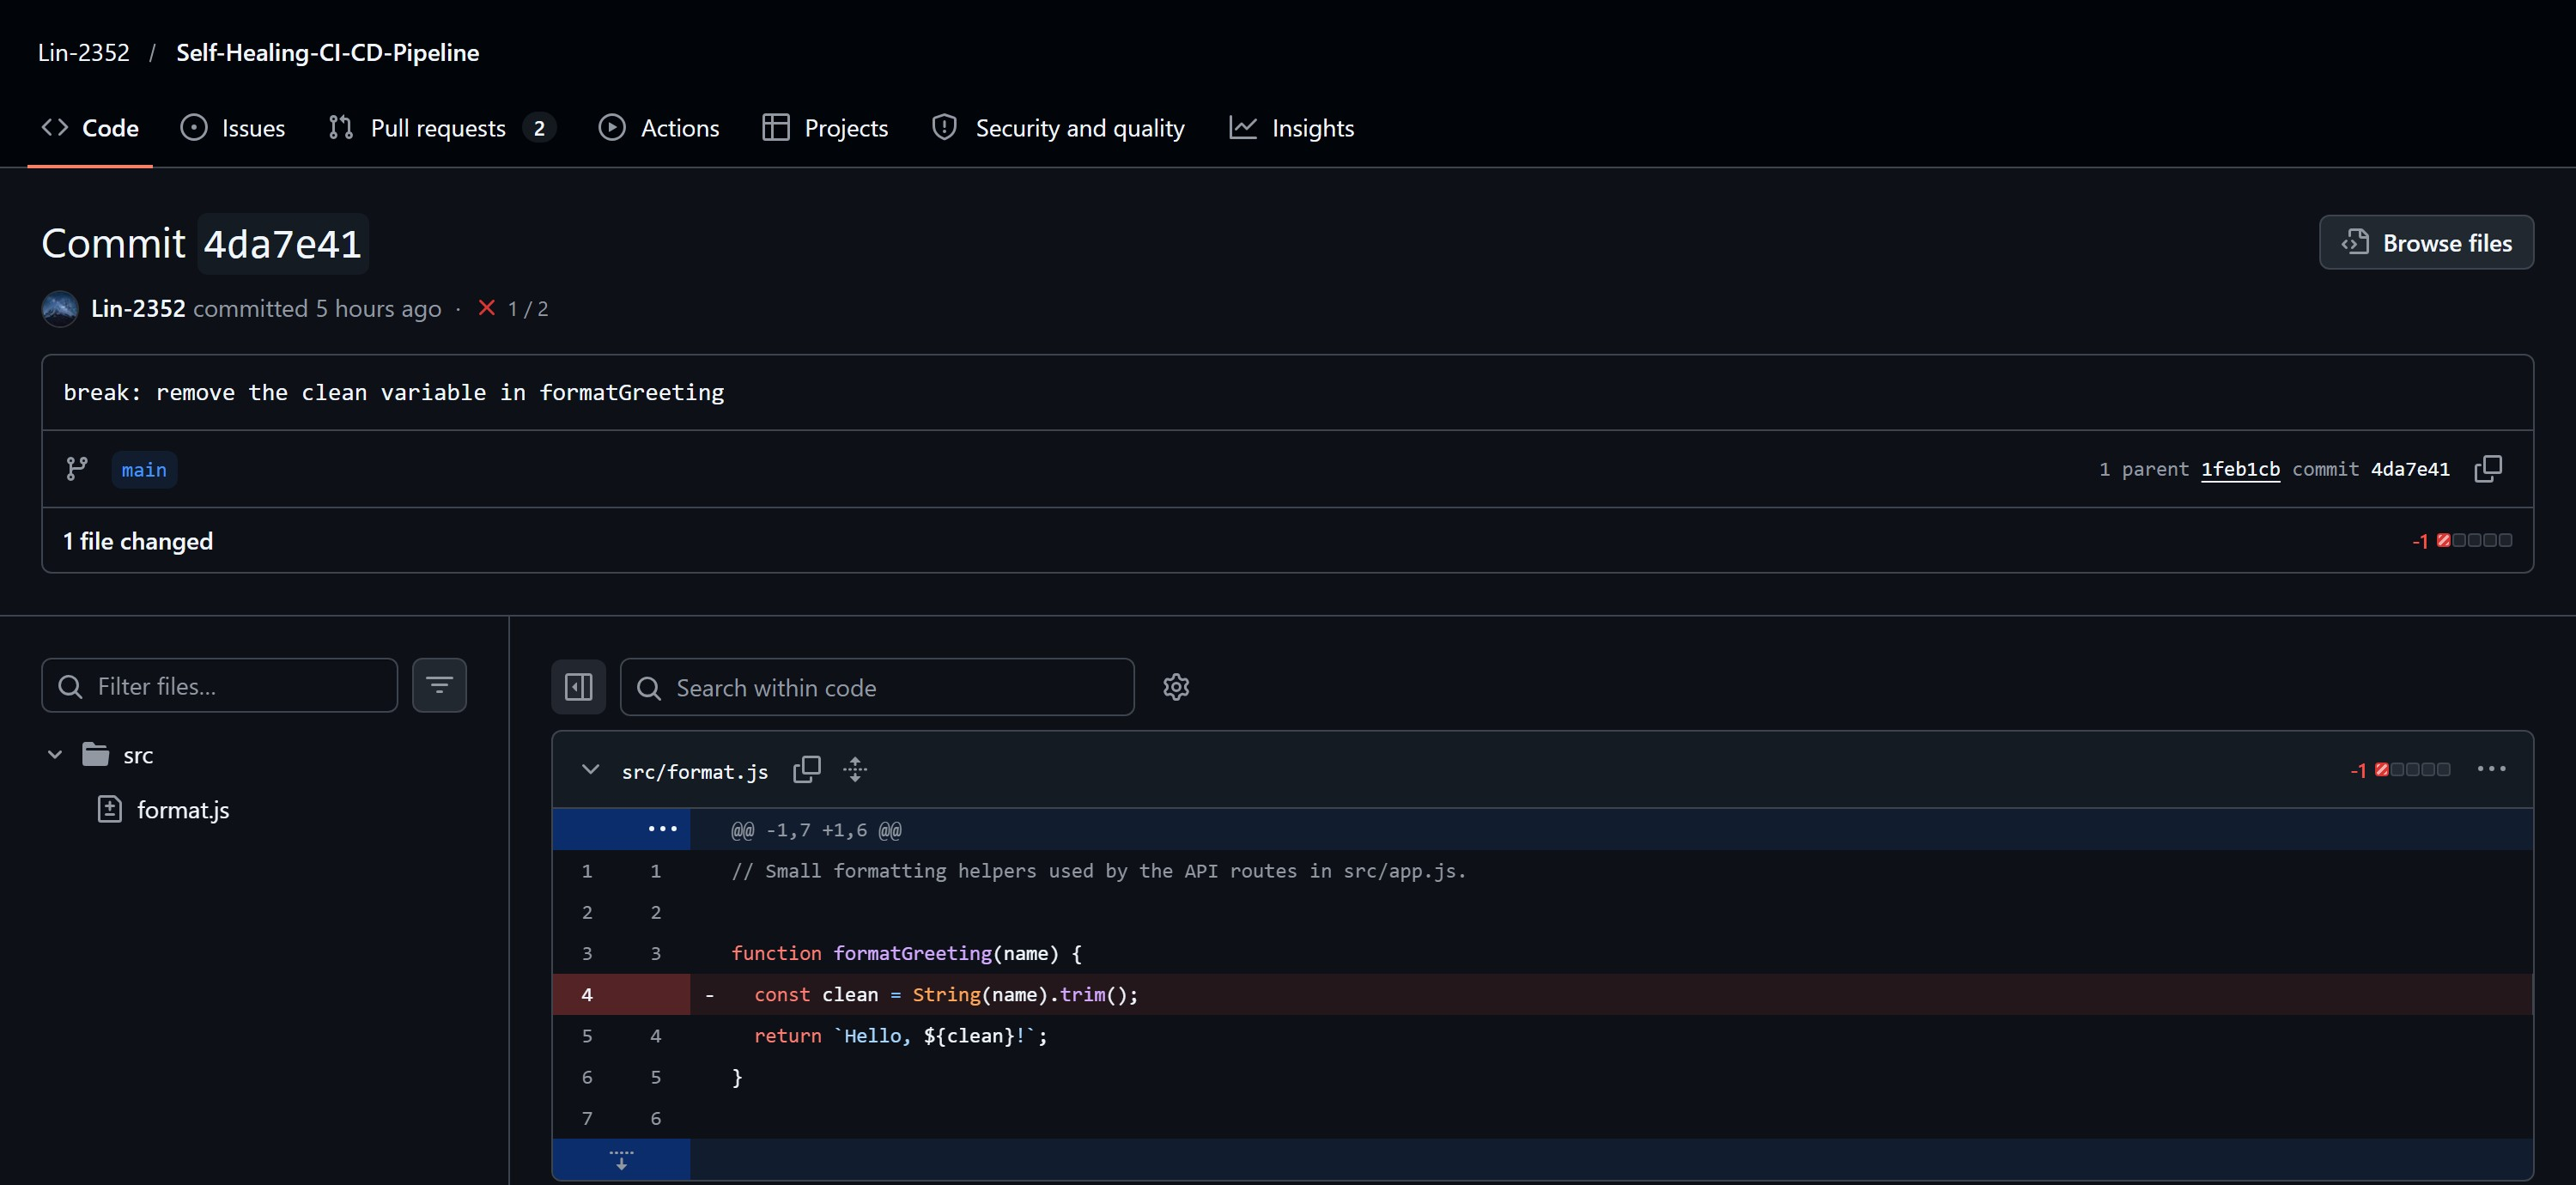
\includegraphics[width=\linewidth]{figures/shots/hq_commit.jpg}
\caption{The breaking commit \texttt{4da7e41}: one line is deleted from \texttt{src/format.js}.}
\label{fig:shot-commit}
\end{figure}
\begin{figure}[!htbp]
\centering
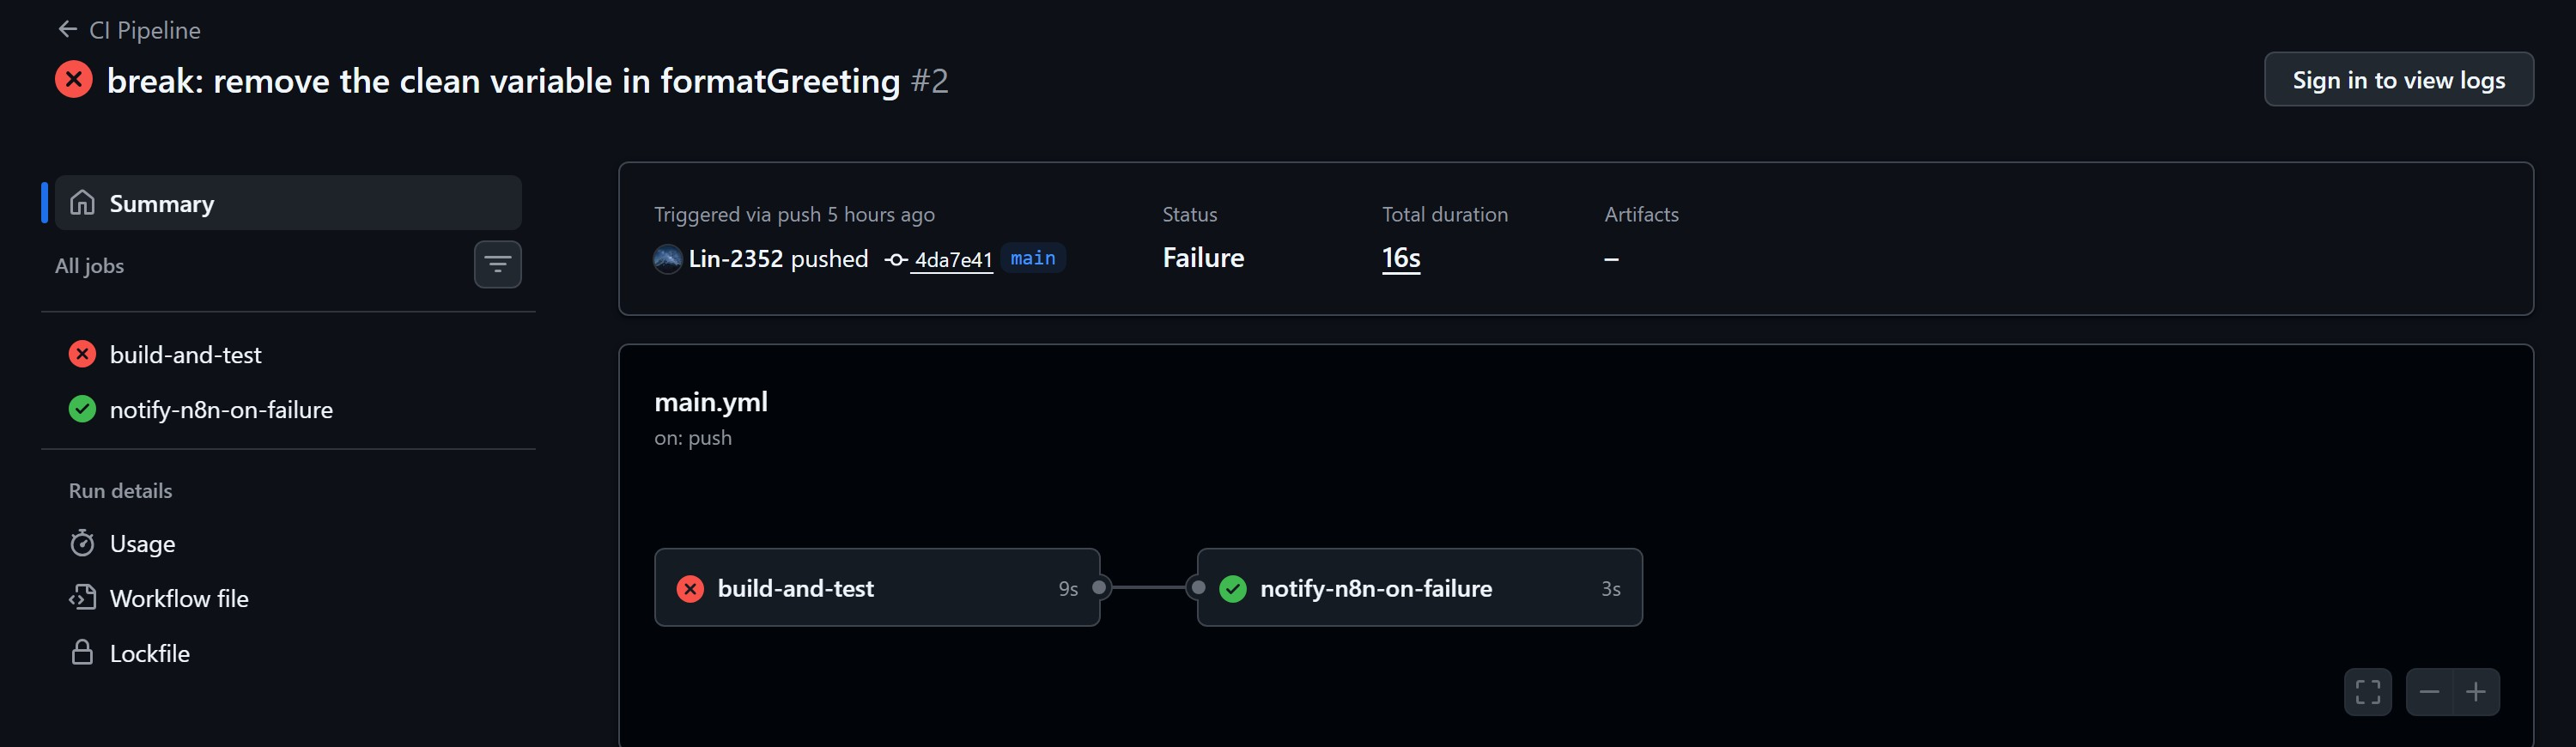
\includegraphics[width=\linewidth]{figures/shots/hq_run.jpg}
\caption{The failing run: \texttt{build-and-test} fails after 9 s, and the \texttt{notify} job that calls n8n passes.}
\label{fig:shot-failed-run}
\end{figure}
\begin{figure}[!htbp]
\centering
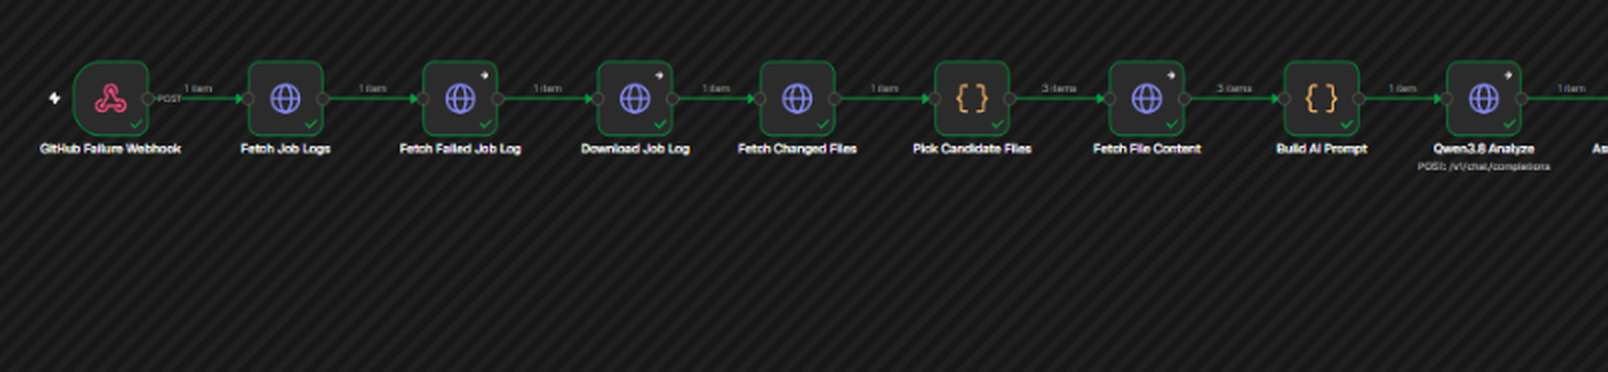
\includegraphics[width=\linewidth]{figures/shots/06a_n8n_left.png}\\[4pt]
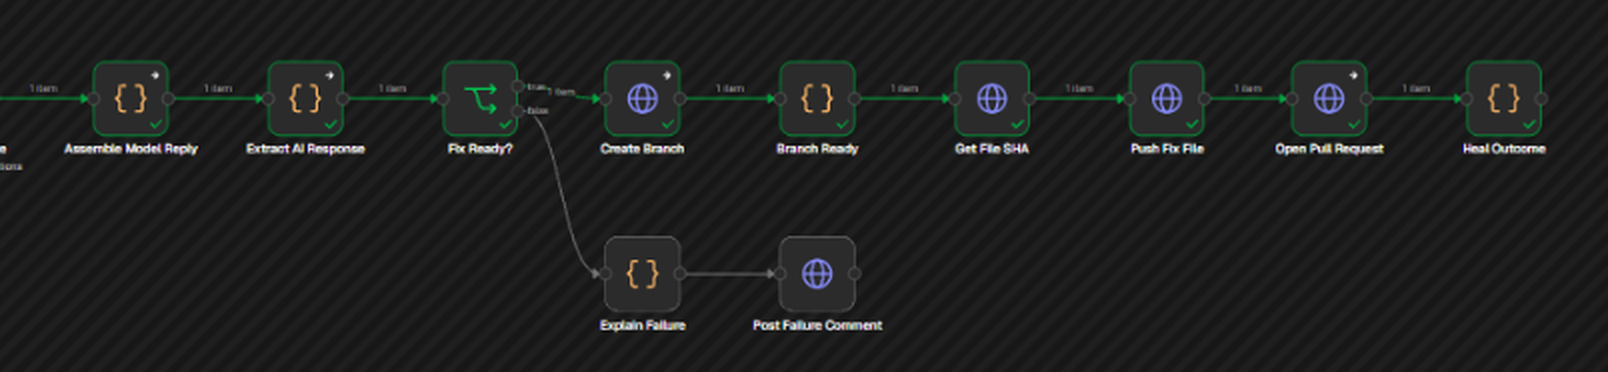
\includegraphics[width=\linewidth]{figures/shots/06b_n8n_right.png}
\caption{The n8n execution of the same run, shown in two halves: every node finished green in 18.7 s.}
\label{fig:shot-n8n}
\end{figure}
\begin{figure}[!htbp]
\centering
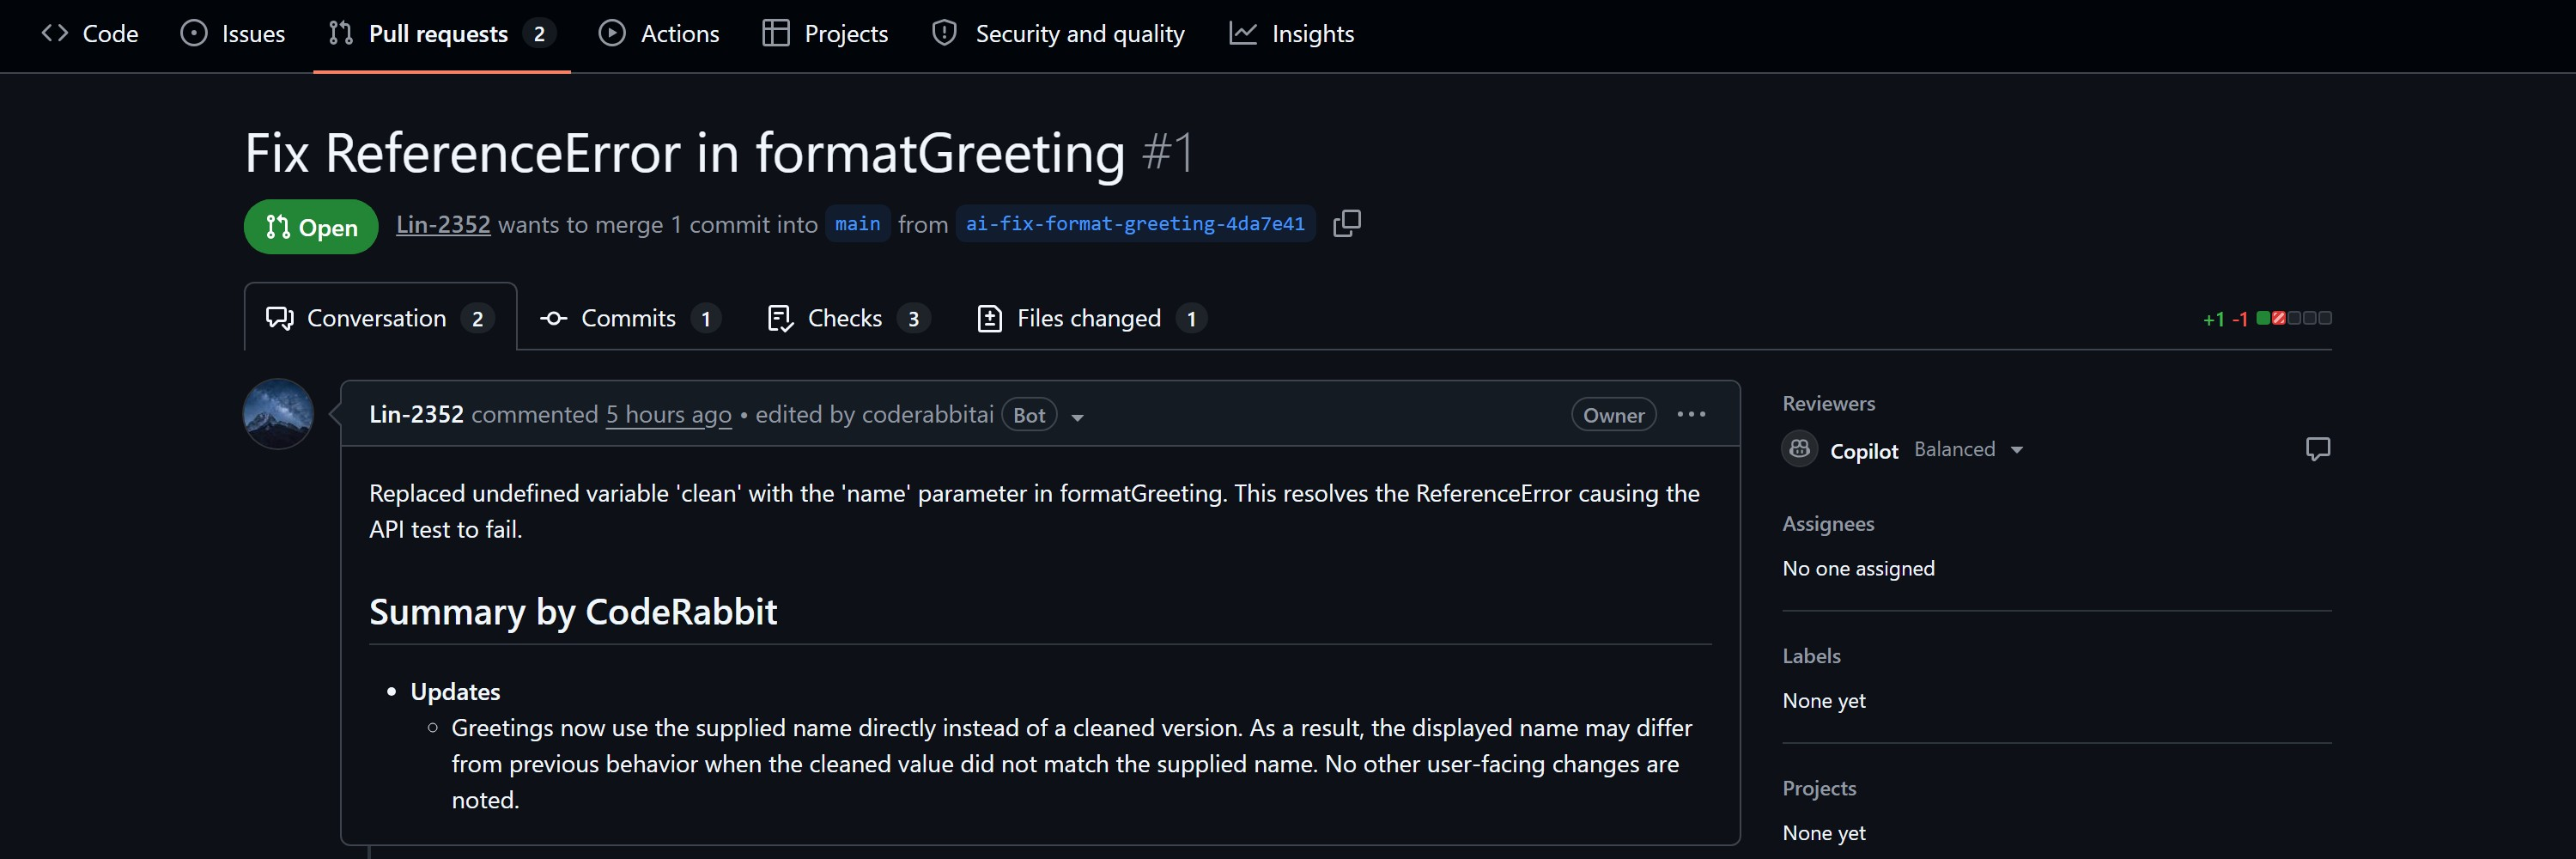
\includegraphics[width=\linewidth]{figures/shots/hq_pr.jpg}
\caption{The pull request opened by the workflow from the branch \texttt{ai-fix-format-greeting-4da7e41}.}
\label{fig:shot-pr}
\end{figure}
\begin{figure}[!htbp]
\centering
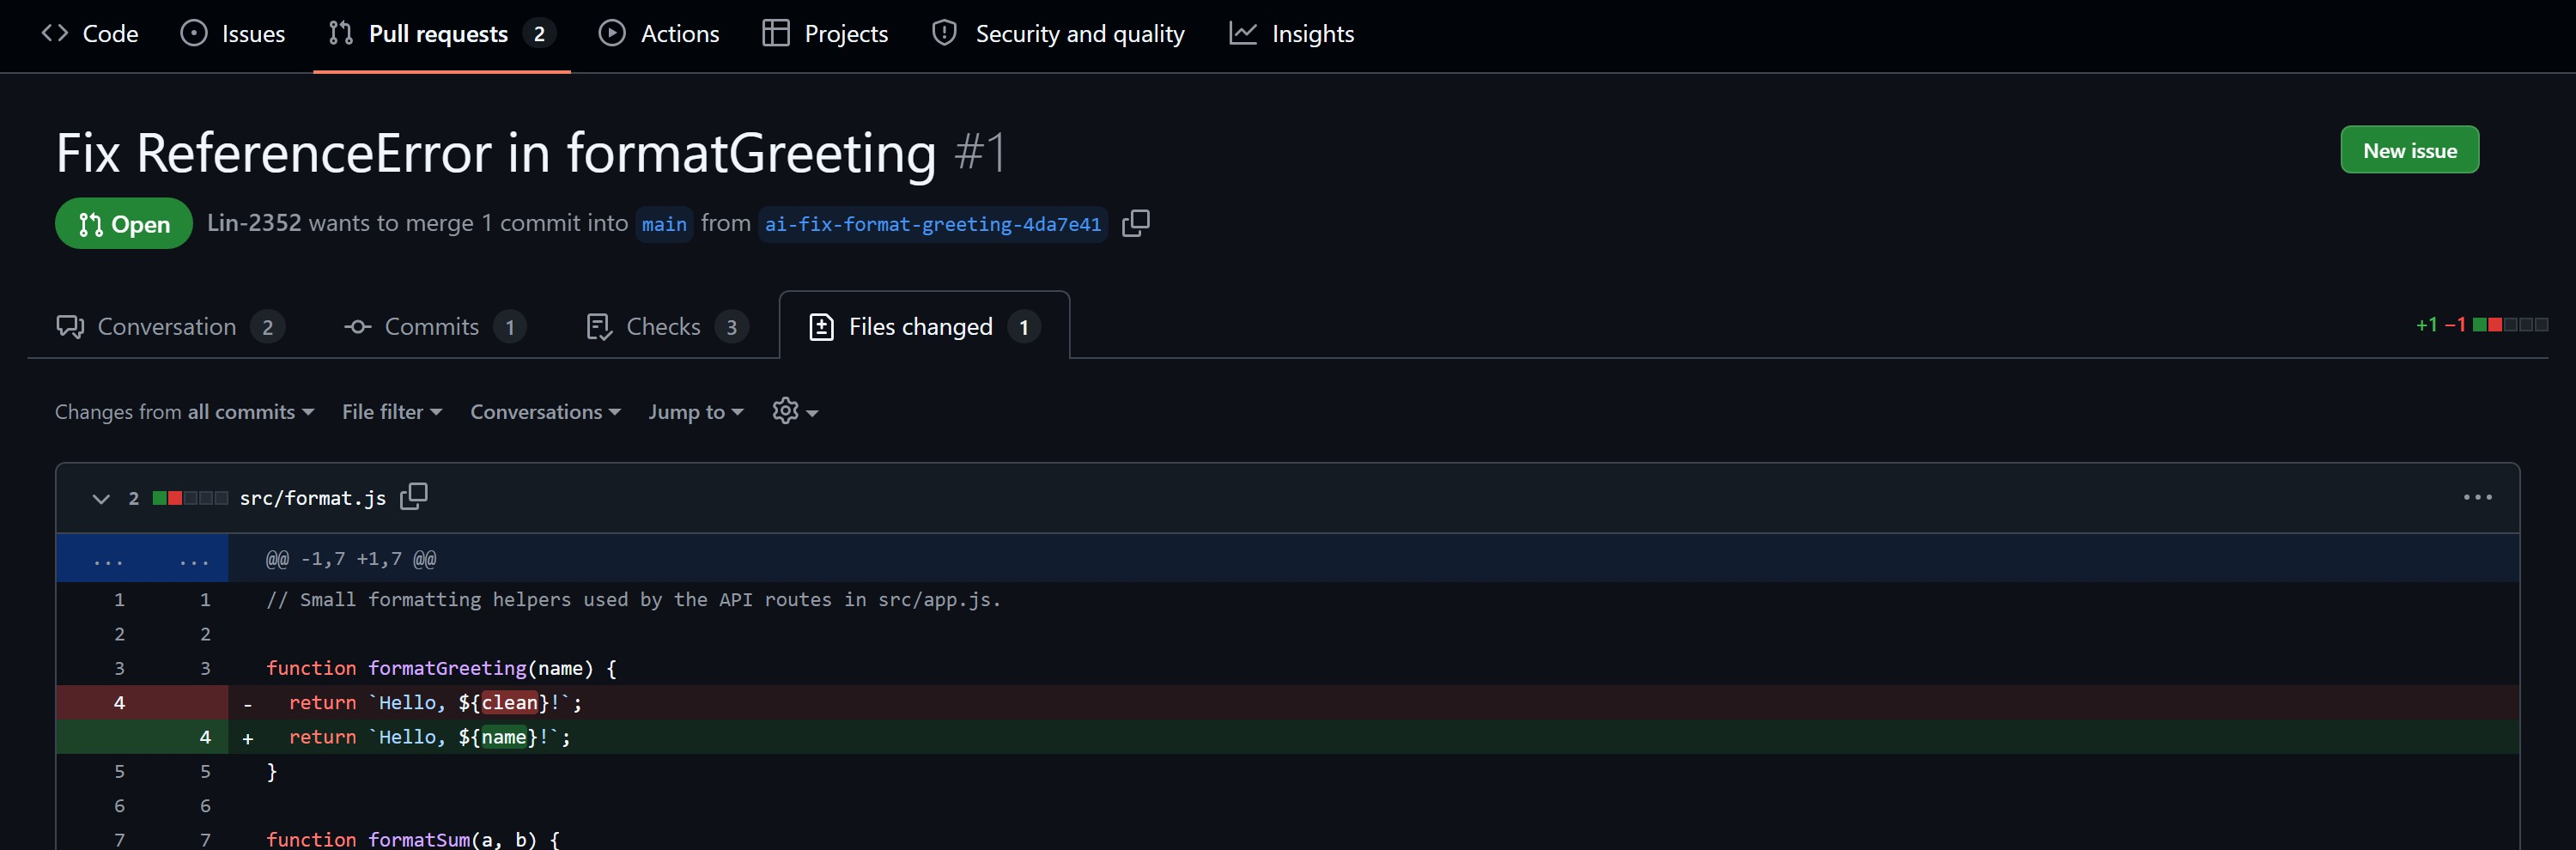
\includegraphics[width=\linewidth]{figures/shots/hq_pr_files.jpg}
\caption{The diff of the pull request: \texttt{\$\{clean\}} becomes \texttt{\$\{name\}}.}
\label{fig:shot-diff}
\end{figure}
\begin{figure}[!htbp]
\centering
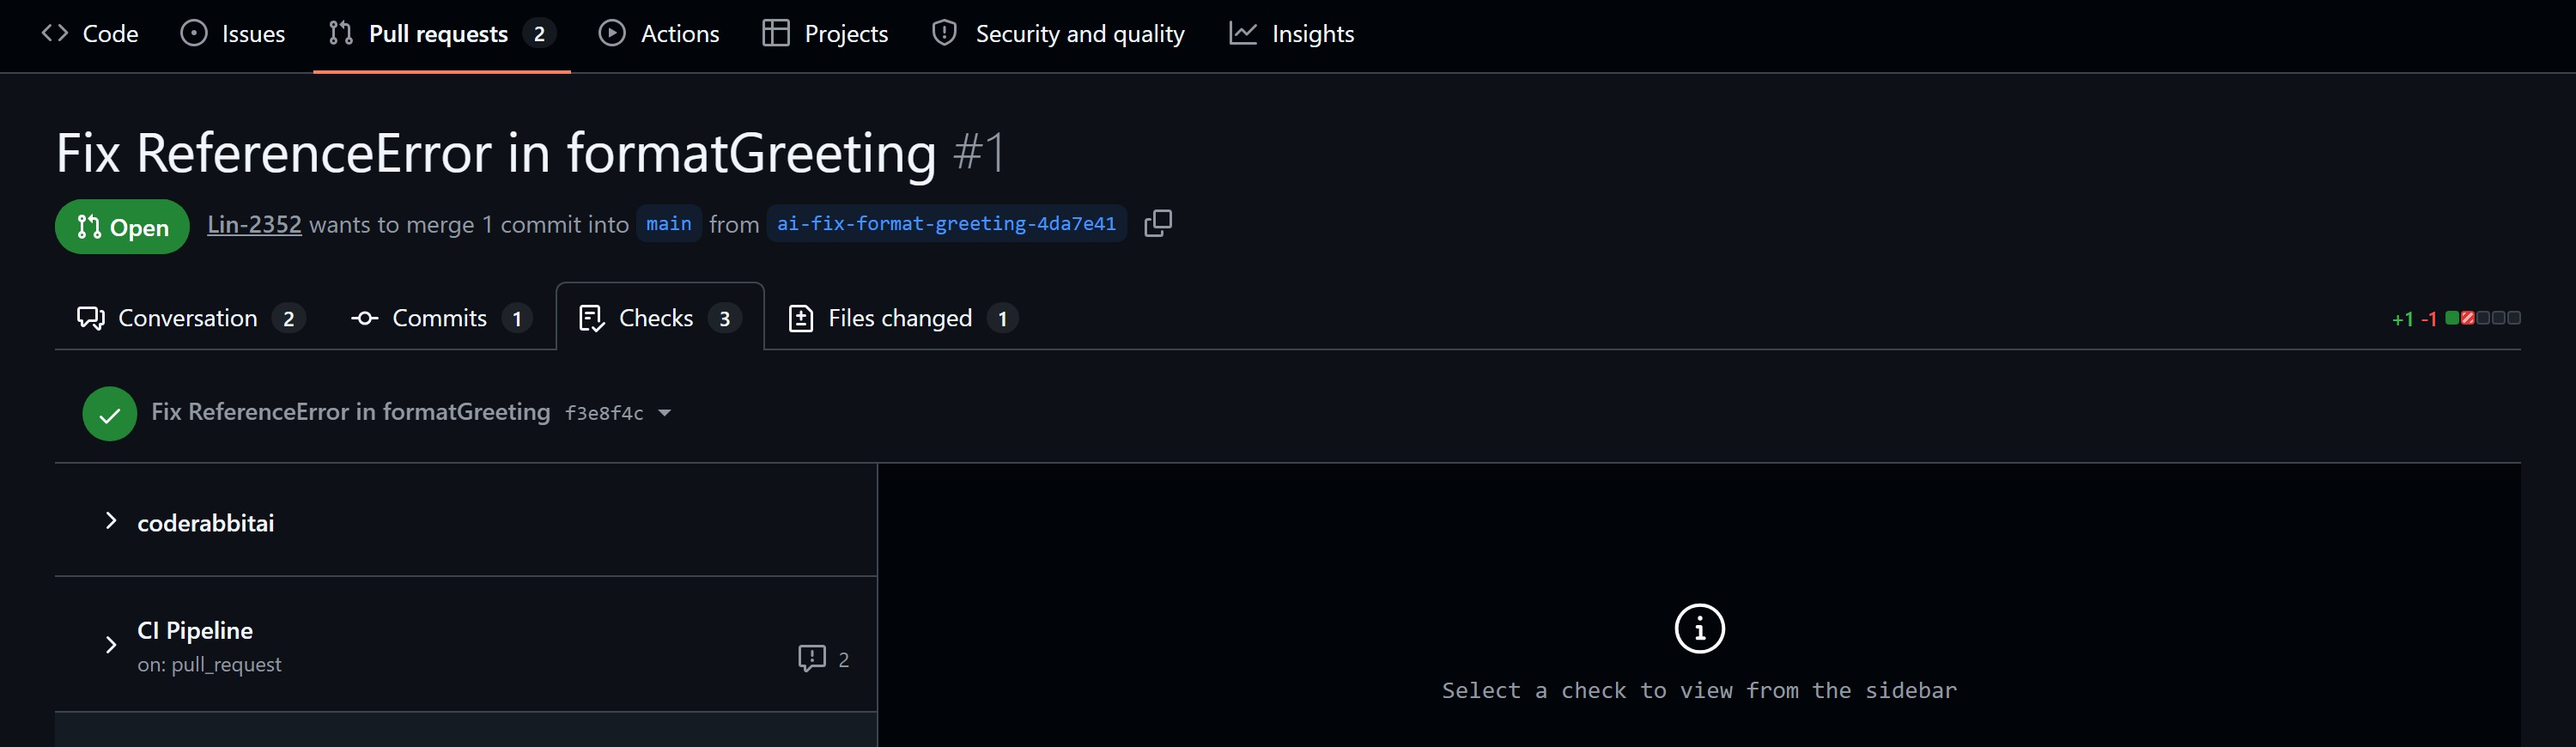
\includegraphics[width=\linewidth]{figures/shots/hq_pr_checks.jpg}
\caption{The checks of the pull request: CI on the fix passes.}
\label{fig:shot-checks}
\end{figure}


\begingroup\small
\begin{longtable}{>{\raggedright\arraybackslash}p{0.071\dimexpr\linewidth-6\tabcolsep\relax}>{\raggedright\arraybackslash}p{0.426\dimexpr\linewidth-6\tabcolsep\relax}>{\raggedright\arraybackslash}p{0.504\dimexpr\linewidth-6\tabcolsep\relax}}
\toprule
\rowcolor{gray!14}\textbf{step} & \textbf{observed} & \textbf{evidence} \\
\midrule
\endhead
\bottomrule
\endfoot
\endlastfoot
1 & The push to \texttt{main} started the workflow run "CI Pipeline \#2". & docs/\allowbreak{}media/\allowbreak{}shots/\allowbreak{}02\_\allowbreak{}actions\_\allowbreak{}runs.jpg \\
2 & \texttt{build-\allowbreak{}and-\allowbreak{}test} failed after 9 s; the run took 16 s in total. The \texttt{notify-\allowbreak{}n8n-\allowbreak{}on-\allowbreak{}failure} job ran and passed after 3 s. & 03\_\allowbreak{}failed\_\allowbreak{}run.jpg \\
3 & The step log shows \texttt{ReferenceError:\allowbreak{} clean is not defined} at \texttt{src/\allowbreak{}format.\allowbreak{}js:\allowbreak{}4:\allowbreak{}20}, then an API test failure, then the line \texttt{npm test exited 1 -\allowbreak{}\textgreater{} failure\_\allowbreak{}kind=code}. & 04\_\allowbreak{}failed\_\allowbreak{}job\_\allowbreak{}log.jpg \\
4 & n8n execution 2 started at 20:45:04, ran 18.699 s and finished with every node green, including all of the branch, push and pull-request nodes. & 05\_\allowbreak{}n8n\_\allowbreak{}execution.jpg, 06\_\allowbreak{}n8n\_\allowbreak{}execution\_\allowbreak{}zoom.png \\
5 & Pull request \#1 "Fix ReferenceError in formatGreeting" opened from the branch \texttt{ai-\allowbreak{}fix-\allowbreak{}format-\allowbreak{}greeting-\allowbreak{}4da7e41} (commit \texttt{f3e8f4c}). & 07\_\allowbreak{}pr\_\allowbreak{}conversation.jpg \\
6 & The diff changes one line: \texttt{\$\{clean\}} becomes \texttt{\$\{name\}}. & 08\_\allowbreak{}pr\_\allowbreak{}diff.jpg \\
7 & CI on the pull request ran 12 s and passed. & 09\_\allowbreak{}pr\_\allowbreak{}checks.jpg, run "CI Pipeline \#3" \\
\bottomrule
\caption{What happened}\label{tab:09arecor-1}\\
\end{longtable}
\endgroup

The breaking commit was pushed at 8:44 PM and the fix pull request's own CI run is listed at 8:45 PM, so the whole chain from push to a passing fix pull request took about a minute on GitHub's minute-resolution timestamps. The two intervals that the pages report to the second are the n8n execution (18.7 s) and the CI run of the fix (12 s).

\subsection{What the run does not show}

The fix is not the original code. The deleted line also converted the value to a string and trimmed it; the model's edit replaces the variable with the raw parameter, so the tests pass while the trimming behaviour is gone. The pipeline's own gates (the SEARCH text matches once, the file parses, CI passes) cannot detect this, which is why the result is a pull request for a person to review, not a merge.

The run used the n8n workflow as it stood before the fallback nodes were added (the execution canvas shows 20 nodes). Later runs on the same repository the same evening used the 26-node version: a run with the model address deliberately set to a dead host went through the OpenAI fallback node, which answered \texttt{Forbidden} (n8n's included free credits did not work for that webhook-triggered run; the cause was not established), and a run after the model address was stored through the Set Model URL webhook healed through Qwen and opened pull request \#2 (execution 6, 17.886 s). The fallback routing is verified by the real-engine tests in Chapter 11; a fix produced by OpenAI has never been observed.

\subsection{A run that could not be repeated}

A second live run for this report was started on 2026-11-15: version 18 of the Kaggle endpoint notebook was pushed and then stayed in the Kaggle queue for about an hour and a half without receiving a GPU. It was cancelled, and the recording above was built from the earlier run, whose pages are still on GitHub and in n8n. Availability of the free GPU is a real operating constraint (Chapter 13).
